\chapter{実装の詳細}

\section{ゲーム環境の実装}
2048は状態からafterstateへの遷移において, 各行~(列)~の変化は独立に考えることができる.
また回転と反転を考慮することで上下左右は等価な盤面変化を起こす.
よって$1$行の全パターンについて, ある一方向を選択したときの遷移先を前もって計算することで, 全方向に対する盤面全体の遷移を高速に行える.

\section{完全解析の実装}
回転・反転に関して同じ盤面は$1$つの状態として扱った.
またそれぞれの状態は$64$ビット整数で表現された.

$3\times3$盤面の2048の完全解析は状態列挙, 価値計算

\section{強化学習の実装}
\subsection{ニューラルネットワークの詳細}
ニューラルネットワークは盤面の特徴量を入力として, 方策と価値を出力する.
盤面サイズ$H \times W$のルールの下では理論上の最高到達タイルは$2^{H \times W + 1}$である.
このとき入力は空きマス$H \times W + 2$チャネルの$H \times W$から成る.
$n$番目のチャネルの$(i,j)$成分には盤面の$(i,j)$
\begin{figure}[t]
    \centering
    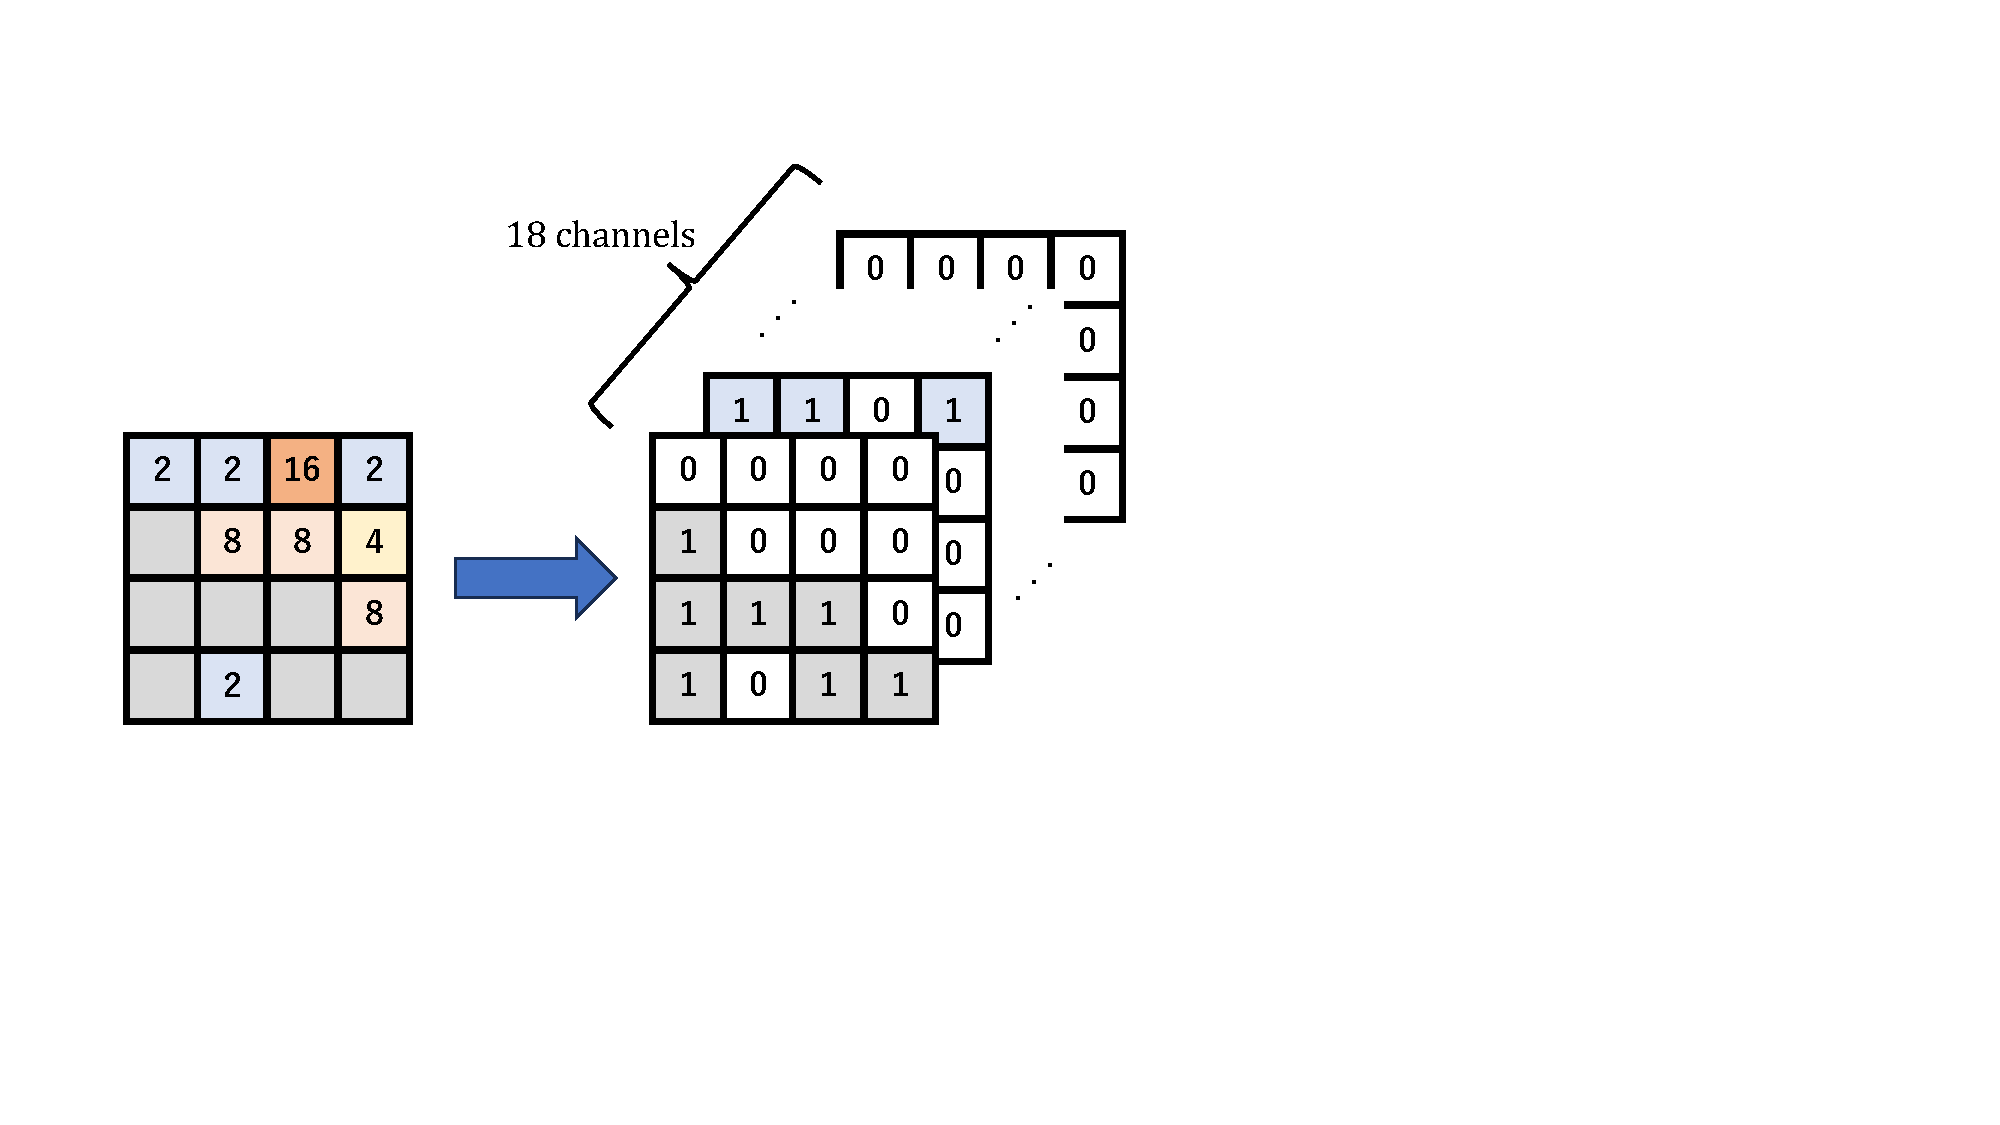
\includegraphics[width=0.6\linewidth{}]{figures/encoding.pdf}
    \caption{ニューラルネットワークへの入力特徴量}
    \label{fig:input_encoding}
\end{figure}

\subsection{AlphaZeroの実装}
ニューラルネットワークは入力に対する方策と価値を出力する.
方策は上下左右それぞれの方向を選択する確率を表す$4$次元のベクトル値である.
価値は

\subsection{Prioritized Experience Replayの詳細}
Prioritized Experience Replay~\cite{prioritized}は学習に使用するデータをランダムではなく, ある重みに従ってサンプルする手法である.
この重みをpriorityと呼び, $i$番目のデータのpriorityは$P(i) = \frac{p_{i}^{\alpha}}{\Sigma_k p_{k}^{\alpha}}$と計算される.
sum treeという二分木でデータを管理することで, $\mathcal{O}(\log n)$に改善することができる.
\begin{figure}[t]
    \centering
    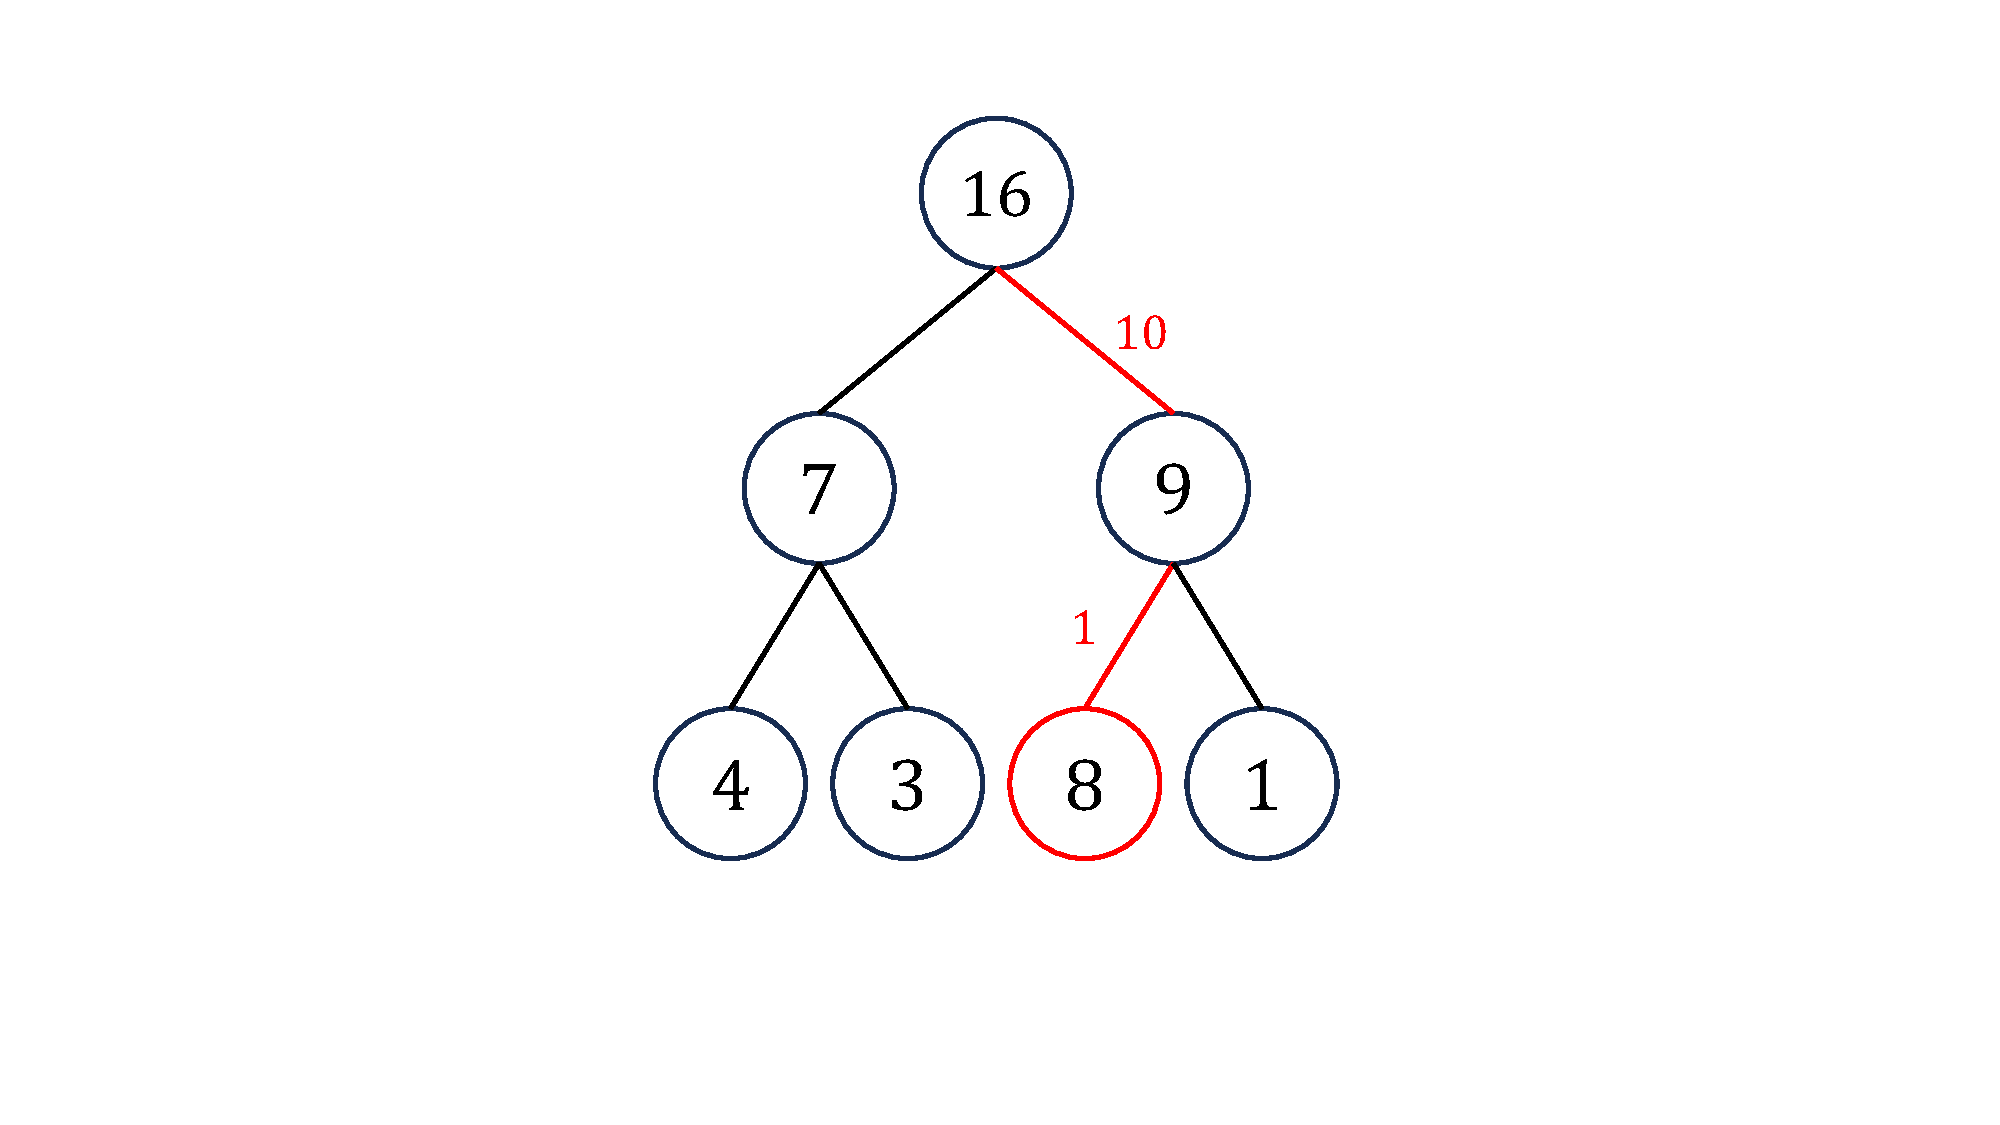
\includegraphics[width=0.4\linewidth{}]{figures/sumtree.pdf}
    \caption{sum treeの例}
    \label{fig:sumtree}
\end{figure}

\chapter{2048のゲーム性とプレイヤの戦略の検証}
\ref{sec:rule}節で述べたように, 2048の通常のルールではafterstateが次の状態へ遷移する際に出現する, 新しいタイルの数字と位置はランダムに決まる.
すなわちafterstateの空きマスから等確率に選択されたある1マスに$90\%$の確率で$2$のタイルが, $10\%$の確率で$4$のタイルが置かれる.

ここで$2$のタイルと$4$のタイルの出現確率を変更した場合にゲーム性がどう変わるか検証する.
表~\ref{table: value_table}に$3 \times 3$盤面の2048において, $4$の出現確率を通常の$10\%$から増減させたときの完全解析の結果を示す.
表から分かるように, $2$と$4$の出現確率がいずれか一方に傾くほど期待値は大きくなる傾向があることが分かる.
また$4$の出現確率が$0\%$の場合と$100\%$の場合には, 最適な行動をし続ければ常に~図\ref{fig:limit}のような理論上の最終盤面に到達できることが分かる.
2048は$2$と$4$の$2$種類の数字タイルが出現することがゲームを面白くしていると考えられる.
\begin{table}[t]
\caption{4の出現確率を増減させたときのゲームの期待値}
\label{table: value_table}
\centering
\begin{tabular}{r|r||r|r}
    \hline 
    4の確率 & 初期状態の期待値 & 4の確率 & 初期状態の期待値 \\ \hline \hline
    0.00 & 7172.00 & 0.55 & 3206.00 \\
    0.05 & 6161.17 & 0.60 & 3171.24 \\
    \textbf{0.10} & \textbf{5468.49} & 0.65 & 3165.36 \\
    0.15 & 4932.54 & 0.70 & 3194.44 \\
    0.20 & 4515.42 & 0.75 & 3269.18 \\
    0.25 & 4182.44 & 0.80 & 3399.20 \\
    0.30 & 3919.20 & 0.85 & 3607.78 \\
    0.35 & 3704.44 & 0.90 & 3993.30 \\
    0.40 & 3531.46 & 0.95 & 4938.20 \\
    0.45 & 3390.19 & 1.00 & 14344.00 \\
    0.50 & 3278.70 &  & \\
    \hline
\end{tabular}
\end{table}

さらに環境が常にプレイヤにとって最も都合の悪くなるように, 新しい数字タイルを出現させるゲームを考える.
これは得点を最大化したいプレイヤと得点を最小化したい環境の対戦ゲームのように考えることができる.
そのため二人零和有限完全確定情報ゲームと同様に, minmax法によってすべての状態の価値$v_{\text{minmax}}$を計算することができる.
具体的には以下の式~\ref{eq:minmax}に従って, ~\ref{sec:solving}節と同様に後退解析を行えばよい.
環境にランダム性がないため, $v_{\text{minmax}}$は常に固定の値をとる.
\begin{align}
    v_{\text{minmax}}(s) =
    \begin{cases}
        0 & (s \text{が終了状態}) \\
        \max_a \left(r(s,a) + \min_{s_\text{next} \in \mathcal{T}(s,a)} v_{\text{minmax}}(s_\text{next}) \right) & (\text{otherwise})
    \end{cases}
    \label{eq:minmax}
\end{align}

さらに$v_{\text{minmax}}$を評価関数として, 通常のルールでプレイさせることを考える.
悲観的な
よってこれをminmaxプレイヤと呼ぶことにする.
一方で常に都合の良い場合を想定して行動する楽観的な戦略も考えられる.
minmaxプレイヤと対比して, これをmaxmaxプレイヤと呼ぶことにする.

次に